%%%%%%%%%%%%%%%%%%%%%%%%%%%%%%%%%%%%%%%%%%%%%%%%%%%%%%%%%
%          File: CascadedTunableFilter.tex            	%
%                  Date: 2 Feb, 2015                	%
%                                                    	%
%   For submission to a journal  						%
%                                                     	%
%   Technical paper about the results obtained with   	%
%   professor Wei Shi with tunable cascaded				%
%	contra-directional coupler				      		%
%	+ theorical analysis								%
%%%%%%%%%%%%%%%%%%%%%%%%%%%%%%%%%%%%%%%%%%%%%%%%%%%%%%%%%

%\documentclass[letterpaper,10pt]{article}
\documentclass[osajnl,twocolumn,showpacs,superscriptaddress,10pt]{revtex4-1}
%\usepackage{osameet2}

%\newcommand{\EDIT}{}
\usepackage{ulem}

\usepackage{amsmath,amssymb}
\newcommand{\me}{\mathrm{e}}
\newcommand*\diff{\mathop{}\!\mathrm{d}}

\usepackage[utf8]{inputenc} %encoding of the input(this text file)
\usepackage[T1]{fontenc} 	%uses the right font encoding
\usepackage{lmodern,textcomp}		%makes font work for fontenc
\usepackage[french,english]{babel} %multiple languages
\selectlanguage{english}	%can switch to french later using this
\usepackage{graphicx,epsfig,epstopdf}
%\usepackage{caption,subcaption}

%\usepackage[numbers]{natbib}
%\renewcommand{\bibfont}{\footnotesize}
%\setlength{\bibsep}{2.0pt}

\begin{document}
\title{Ultra-compact, widely bandwidth-tunable filter using cascaded silicon photonic contra-directional couplers}
%\date{14/10/2014}

\author{Jonathan St-Yves} 
\author{Hadi Bahrami}
\author{Philippe Jean}
\author{Sophie Larochelle}
\author{Wei Shi}\email{Corresponding author: wei.shi@gel.ulaval.ca}
\affiliation{Centre d'optique, photonique et laser (COPL) and Département de génie électrique et génie informatique, Université Laval, 2375 rue de la Terrasse, Québec (Québec), Canada, G1V 0A6}


\begin{abstract}
We demonstrate an integrated silicon tunable band-pass filter with low in-band ripples of 0.3 dB, a high contrast of 55 dB, and no free-spectral range. 
A record bandwidth tuning from 788 to 117 GHz was achieved.
\end{abstract}

\pacs{ (130.7408) Wavelength filtering devices; (350.2770) Gratings}

%\linespread{0.95}		%Space saving emergency line

\maketitle

%\section{Introduction}


%Next-generation optical transmission systems require dynamic, efficient bandwidth allocation  
%Bandwidth tunable optical filters are essential components for optical communication applications such as reconfigurable optical wavelength-division multiplexing (WDM), signal processing, and dynamic bandwidth allocation \cite{DynamicBW}.
%These key devices are now needed in integrated photonic systems, in this case, on the silicon-on-insulator platform (SOI), to achieve the same functions as traditional discrete optical components such as diffractive grating spectrometers. 
Next-generation optical transmission systems applying flexible networking and the super-channel technique will require highly dynamic channel allocation to drastically increase the spectral efficiency and transmission capacity \cite{jinno2009spectrum, geisler2011demonstration}.
%over a few hundred gigahertz \cite{jinno2009spectrum}. 
%bandwidth
Tunable optical filters, reconfigurable in both center wavelength and bandwidth with scalability towards terahertz \cite{geisler2011demonstration}, are essential for these applications.
Such large bandwidth tunability is currently only available in bulky bench-top systems using diffractive grating spectrometers or liquid crystals.
Integrated solutions are desired for lower cost and power consumption.
In particular, silicon photonics  based on the submicron silicon-on-insulator platform allows for CMOS compatible mass fabrication, enabling low cost, high yield, and high-density chip-scale integration.
Existing solutions for tunable  filters on silicon include devices based on microring resonators \cite{DynamicBW, ong2013ultra} and Mach-Zehnder interferometers (MZIs). These devices have relatively small tunable bandwidth (less than 200 GHz) and small free spectral ranges (FSRs) (typically less than 10 nm), not suitable for high-capacity transmission applications.

Contra-directional couplers(contra-DCs) are grating-assisted add-drop filters \cite{shi2013siliconContraDC}. 
Analogous to waveguide Bragg gratings, the wavelength selectivity in contra-DCs are based on periodic dielectric perturbations. But instead of backreflections in the same waveguide, the selected wavelength in a contra-DC is dropped to another waveguide through contra-directional coupling.
This allows add-drop operation without the need of a circulator. 
Contra-DCs have merits of compactness, flat-top response, flexible filter design (e.g, through apodization), and near-infinite FSR (in the case of first-order gratings).
In particular, they allow for very high bandwidths (greater than 10 nm) and thus can support very-high-baud-rate super-channel signals \cite{jinno2009spectrum}.
In this paper, we demonstrate a broadband filter with a large tunability in both wavelength and channel bandwidth, using thermally controlled cascaded contra-DCs on a silicon chip. 
The filter has flat-top responses, low insertion loss, low in-band ripples, and high contrast between the pass-band and the stop-band.

\begin{figure}[htbp]
	\centering
	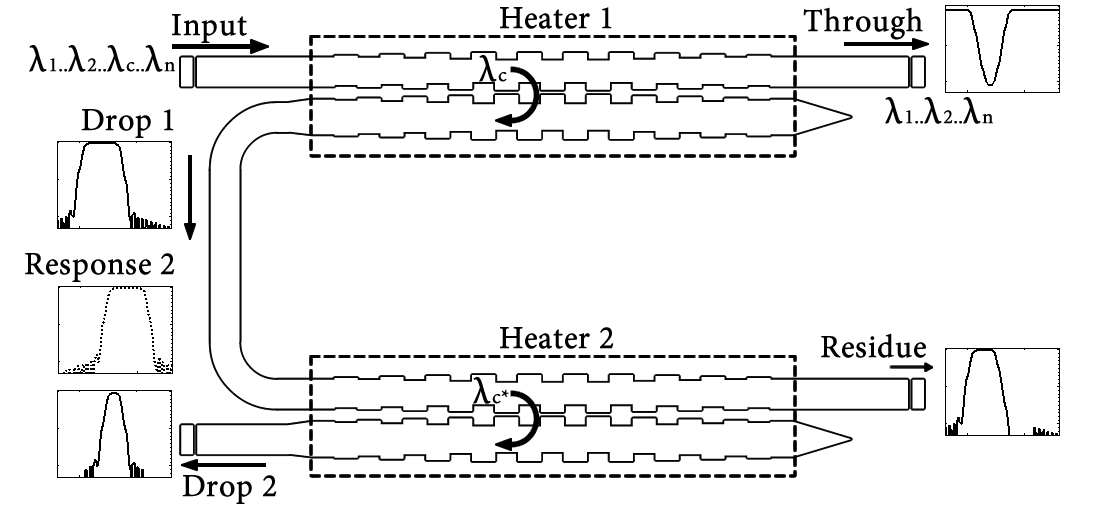
\includegraphics[width=1.00\columnwidth]{data/CascadedSchematic2}
	\centering
	\caption{Schematic of the device. 
	The dropped wavelength of the first contra-directional coupler is re-filtered in an identical component. 
	Both contra-directional couplers are temperature-controlled with metal heaters. 
	Plots show examples of spectrum at each port, on a logarithmic scale.}
	\label{fig:schematic}
\end{figure}
%\section{Principle and Design}

The schematic of the proposed device is shown in Fig.~\ref{fig:schematic}. 
It consists of a pair of cascaded contra-DCs, each operating as an add-drop filter. 
The drop port of the first contra-DC is connected to the input port of the second contra-DC. 
Therefore, the finally dropped signal is determined by the product of the  drop-port transfer functions of the two contra-DCs. The center wavelength of a contra-DC is determined by the phase-match condition: $\lambda_\text{c} = \Lambda (n_\text{1}+n_\text{2})$, where $\lambda_\text{c}$ is the center wavelength of contra-directional coupling, $\Lambda$ is the grating pitch, and $n_\text{1}$ and $n_\text{2}$ are the effective refractive indices of the first-order and second-order eigenmodes in the coupler. 
Assuming identical filter designs (i.e., same window functions and parameters) of the cascaded contra-DCs, the bandwidth of the finally dropped signal can be tuned by detuning their center wavelengths.



\begin{figure}[htbp]
  \centering
  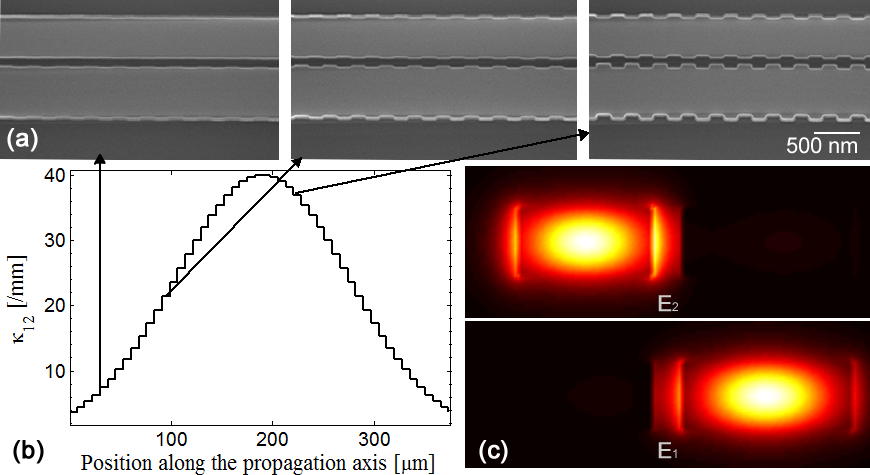
\includegraphics[width=1\columnwidth]{data/FigApod}
  \caption{(a)SEM photography of a part of the grating. The contra-directional coupler consists of two close waveguides of different width with periodic sidewall corrugations. (b) Apodization profile of the grating. A larger coupling requires larger corrugations. (c) Intensity distributions of electrical fields of the first and second transverse modes. }
  \label{fig:SEM}
\end{figure} 


A broadband filter design for a coarse WDM on the 220-nm SOI platform \cite{shi2013siliconCWDM} is adopted for individual contra-DCs.  
In each contra-DC, the widths of the waveguides are of 560 and 440 nm.
This high asymmetry ensures a negligible forward coupling. 
The gratings are formed by sidewall corrugations in strip waveguides with a pitch of 312 nm. 
The spacing between the waveguides varies between 65 and 135 nm with a Gaussian profile as shown in Fig.~\ref{fig:SEM} for efficient sidelobe suppression, for which details can be found in \cite{shi2013siliconCWDM}.
The spectral responses of each contra-DC is calculated using coupled mode theory, following the same procedure as in  \cite{shi2013siliconContraDC}, with three additions: apodization, temperature and noise simulation.

%The first part in predicting the contra-directional coupler spectrum is to compute the dielectric variation caused by the perturbation $\Delta\varepsilon(x,y)$ which is $\varepsilon_0/\pi*(n_{max}(x,y)^2-n_{min}(x,y)^2)$ where the $1/\pi$ factor is the first Fourier expansion coefficient in the case of a square shaped perturbation. 
%One also needs the mode distribution in each waveguide  $E_1(x,y)$ and $E_2(x,y)$ at the average point of the perturbation, which can be obtained using a 2D eigenmode solver such as Lumerical MODE. 
%The couplings $\kappa_{11}$, $\kappa_{12}$ and $\kappa_{22}$  can then be calculated from
%\begin{equation}\label{eq:coupling}
%\kappa_{nm}=\frac{\omega}{4}\iint \textbf{E}^*_n(x,y)\Delta\varepsilon_1(x,y) \textbf{E}_m(x,y) \diff x \diff y
%\end{equation}

While an unapodized (uniform) grating can be simulated with only two transfer matrices , $S_1$ and $S_2$ \cite{shi2013siliconContraDC}, an apodized one needs both of these matrices for each step along the propagation, to match the change of coupling. 
The first change is thus to modify the transfer matrix of the system to the product of all the grating elements along the propagation axis.
This calculation ideally takes shape in an infinite sum, but for computation simplicity, we use a finite number of steps with different couplings that still approximates the apodization profile with enough accuracy. 
Our simulations uses  steps of constant length $z_i-z_{i-1}=z_c$. 
%The total response of a contra-DC $C(z_0,z_n)$ is calculated using the transfer-matrix method, where $E(z_0)=C(z_0,z_n) E(z_n)$.

%\begin{equation}
%\label{eq:CMatrix}
% C(z_0,z_n) =  \prod_{i=1}^{n}\me^{S_{1,i}(z_i-z_{i-1})}\me^{S_{2,i}(z_i-z_{i-1})}
%\end{equation}

%with $\Delta\hat{\beta}_{1,2} = \frac{2\pi}{\lambda}n_{\text{eff }1,2}-\frac{\pi}{\Lambda}$ and

%\begin{equation}
%S_1= \begin{bmatrix}
%		j\Delta\hat{\beta}_1 & 0 & 0 & 0 \\
%		0 & j\Delta\hat{\beta}_2 & 0 & 0 \\
%		0 & 0 & -j\Delta\hat{\beta}_1 & 0 \\
%		0 & 0 & 0 & -j\Delta\hat{\beta}_2
%	 \end{bmatrix}
%\ end{equation}

%\begin{figure*}[tbp]
%
%\begin{equation}
%\begin{split} 
%S_2= 
%\begin{bmatrix}
%-j\Delta\hat{\beta}_1 & 0 & -j\kappa_{11}\me^{j2\Delta\hat{\beta}_1 z_c} & -j\kappa_{12}\me^{j(\Delta\hat{\beta}_1+\Delta\hat{\beta}_2) z_c} \\
%0 & -j\Delta\hat{\beta}_2 & -j\kappa_{12}\me^{j(\Delta\hat{\beta}_1+\Delta\hat{\beta}_2) z_c} & -j\kappa_{22}\me^{j2\Delta\hat{\beta}_2 z_c} \\
%j\kappa^*_{11}\me^{-j2\Delta\hat{\beta}_1 z_c} & j\kappa^*_{12}\me^{-j(\Delta\hat{\beta}_1+\Delta\hat{\beta}_2) z_c} & j\Delta\hat{\beta}_1 & 0 \\
%j\kappa^*_{12}\me^{-j(\Delta\hat{\beta}_1+\Delta\hat{\beta}_2) z_c} & j\kappa^*_{22}\me^{-j2\Delta\hat{\beta}_2 z_c1} & 0 & j\Delta\hat{\beta}_2
%	 \end{bmatrix}
%\end{split} 
%\end{equation}
%\hrulefill
%\end{figure*}

It is possible to easily add phase noise to the transfer matrix solution by adding random noise to the $\Delta\hat{\beta}$ propagation constants. The frequency distribution of the noise will thus match the quantization steps of the matrices, but since the response noise is dependent of both the amplitude and frequency of the sidewall roughness \cite{simard2011impact},we can match the simulation to the experiment by choosing the right noise amplitude.


On top of each contra-DC sits a metal strip acting as a microheater for thermal tuning.  
The refractive index of silicon has a temperature dependence of $\frac{\diff{n_\text{Si}}}{\diff{T}}=$ 1.87$\times10^{-4}$K$^{-1}$ at room temperature for wavelengths around 1550 nm~\cite{frey2006temperature}.
Without electrical input, the optical responses of the two filters are identical (neglecting fabrication uniformities) resulting in a sharp transition from the pass-band to the stop-band. 
Applying independent electrical currents on the heaters, we can shift the spectra of the contra-DCs simultaneously or differentially for wavelength or bandwidth tuning.
In the ideal case, each contra-DC should be uniformly heated so that the apodization profile isn't disturbed as the temperature varies.

In simulation, the temperature dependence is accounted for by increasing the effective index according to 
$\diff{n_\text{eff}}=\frac{\diff{n_\text{Si}}}{\diff{T}}*\frac{\diff{n_\text{eff}}}{\diff{n_\text{Si}}}*\diff{T}$, where $\frac{\diff{n_\text{eff}}}{\diff{n_\text{Si}}}$ is calculated using an eigenmode solver.




%\section{Experiment}

The device was fabricated using a CMOS-compatible technology with electron-beam lithography. 
Fiber grating couplers\cite{zhong2014focusingFGC} were used as optical IOs in the measurement. 
Fig.~\ref{fig:passive} shows the measured drop port response of the cascaded contra-DC filters. 
The measurements were normalized using the response of a pair of directly connected fiber grating couplers on the same chip.
\begin{figure}[htbp]
\centering
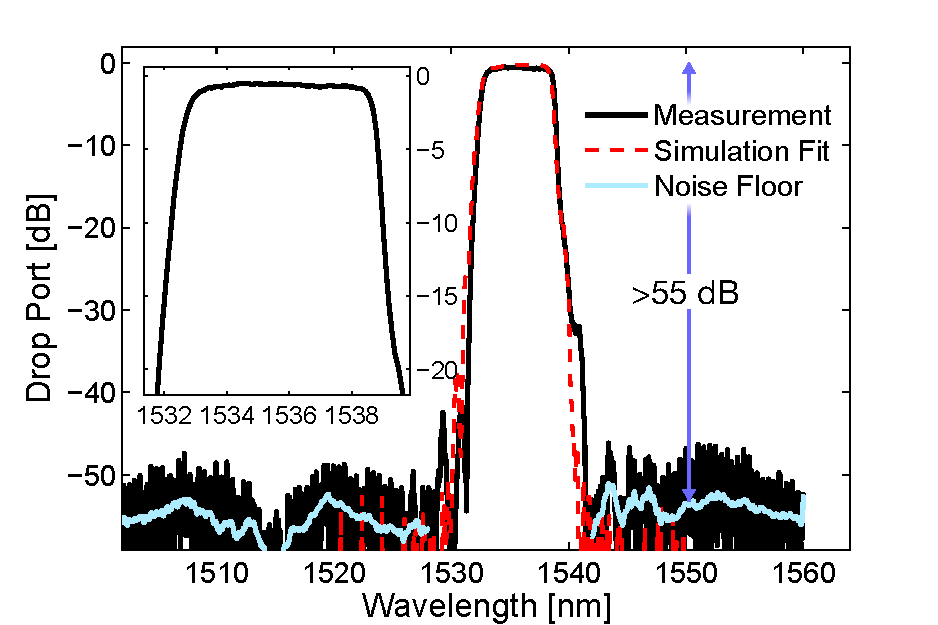
\includegraphics[width=.99\columnwidth]{data/Passive6}
\caption{ Spectral response of the cascaded filters without heating: 1-dB BW is 733 GHz, 3-dB BW is 788 GHz, 10-dB BW is 868 GHz, and 20-dB BW is 990 GHz. Inset shows the filter shape up to -20 dB, which is the typical communication requirement.}
\label{fig:passive}
\end{figure}

The device exhibits a high side-lobe suppression ratio (SLSR) of over 40 dB and a high contrast of about 55 dB between the pass-band and the stop-band. 
The insertion loss is very low, less than 0.5 dB (i.e., 0.25 dB per contra-DC), with small ripples of less then 0.3 dB within the 1-dB passband over 5.8 nm (733~GHz). 
The edge roll-off rate is 19 dB/nm on the left side and 24 dB/nm on the right side.
Further work could optimize the grating structure using the inverse layer peeling algorithm\cite{skaar2001synthesis} since the mathematics of the contra-directional coupler are similar to those of Bragg gratings.

By changing the temperature of a single contra-DC, we offset the phase-match condition of a filter, resulting in a smaller band overlap between the two contra-DCs and thus a narrower passband in the drop port, as shown in Fig.~\ref{fig:bandTune}.  
Due to the wavelength detuning,  the stop-band edges are only determined by the single filters. 
As a result, the side-lobes suppression degrades  for small bandwidths but is still better than 15 dB. A continuous tuning of the 3-dB bandwidth from 788 GHz down to 117 GHz (i.e., over 670 GHz or 5.4 nm) is experimentally observed as the on-chip temperature increases by 70 degrees. 
The smallest bandwidth measured in this case was limited by the maximal power delivered before the metal heaters (300-nm-thick, 2-$\mu$m-wide Al strips) were damaged. A smaller bandwidth below 50 GHz should be feasible if more robust heaters are used.
The power efficiency of the bandwidth tuning is about 24 mW/nm, which can significantly improved by optimizing the heater design, e.g., using smaller heater features and thermal isolation \cite{dong2010thermally}.

\begin{figure}[htbp]
\centering
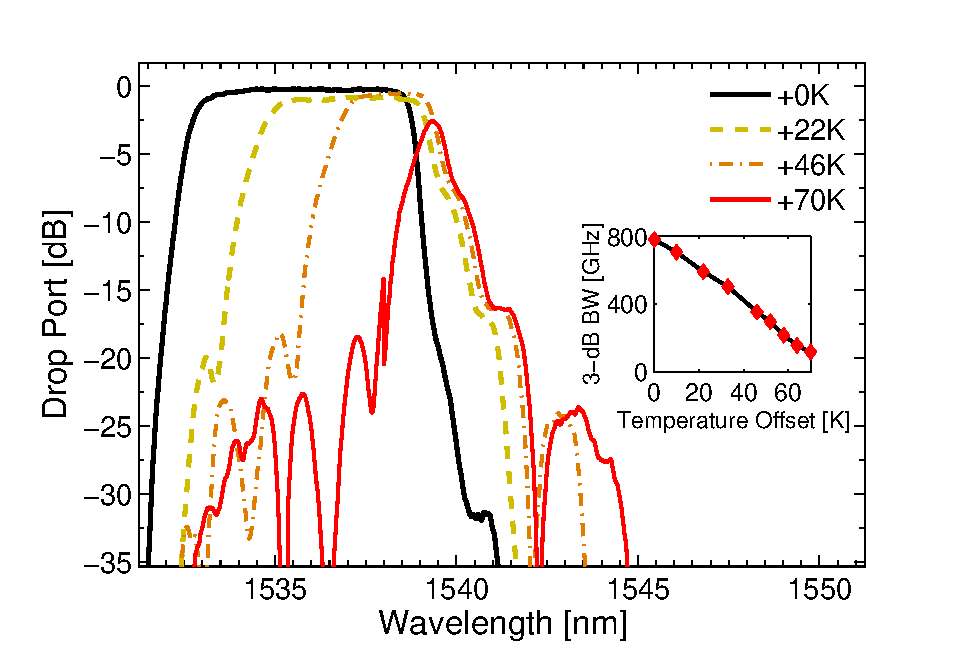
\includegraphics[width=.99\columnwidth]{data/Band6}
\caption{Spectral response of the device for different temperatures applied to only one contra-DC: 1-dB BW tuned down to 65 GHz, 3-dB BW to 117 GHz. The temperatures are obtained from simulation fit. Inset shows the temperature dependence.}
\label{fig:bandTune}
\end{figure} 

By applying the same temperature variation on both contra-DCs, the center wavelength can be tuned without affecting the filter shape.
As shown in Fig.~\ref{fig:wavTune}, when the center wavelength is continually changed over 4 nm by varying the on-chip temperature, the filter shape is maintained with sharp edges. Actually, slight detuning between the cascaded contra-DCs may be used to compensate for band-edge distortions due to fabrication errors for a more symmetric filter shape. 
The power efficiency of the wavelength tuning is about 44 mW/nm, which is about twice the power consumption of the bandwidth tuning since two contra-DCs are heated simultaneously.
\begin{figure}[htbp]
\centering
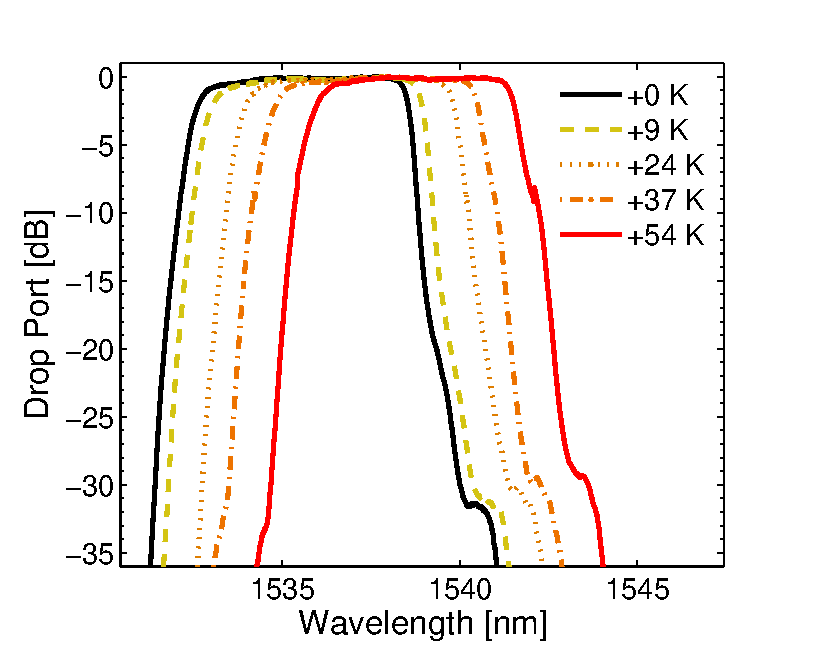
\includegraphics[width=.99\columnwidth]{data/Central2}
\caption{Spectral response with the heat applied to both contra-DCs: the central wavelength is tuned from 1535 nm to 1539 nm continuously; the temperatures are calculated by comparison to simulation. Inset shows the temperature dependence.}
\label{fig:wavTune}
\end{figure} 


%\section{Theoretical Performance Limits}

%\subsection{Out of band rejection ratio}
%Limited by \textbf{Apodisation} and Phase Noise.
%A contra-directional coupler spectrum will contain sidelobes corresponding to the Fourier transform of the coupling profile along the propagation axis. 
%Using a constant coupling is analogous to a rectangular window, causing sidelobes of over -15 dB. 
%The use of a Blackman–Nuttall or similar high-order gaussian coupling profile theoretically reduces the sidelobes amplitude to under -50 dB, although electron beam grid resolution distorts the profile by forcing discrete coupling values.

%Still, the dominant cause of weak out of band rejection ratio is phase noise due to sidewall roughness\cite{simard2011impact}. The random change of waveguide width causes the effective index of the modes to jitter, causing a variation of the Bragg-wavelength.

%Both of these effects are added to our simulation using a transfer matrix method. 
%First, multiple matrices are used along the propagation length, with couplings corresponding to the apodization profile.
%Second, the effective index in each of these matrix is randomly varied by an amount corresponding to the roughness amplitude.
%Since the effect of phase noise is dependent on it's spacial frequency \cite{simard2011impact}, and this frequency is based on the matrix discreteness, the simulation noise is calibrated using measurements data.

%As seen in this experiment however, it is possible to greatly improve the out of band rejection ratio by cascading multiple filters together, which adds up the rejection ratio of each, at the cost of making the device longer

%\subsection{In-band insertion loss}
%Limited by length and sidewall roughness loss. 
%The insertion loss in each device at 1550 nm is mainly caused by the material absorption of silicon and scattering loss due to sidewall roughness. 
%The most important parameter to optimize losses is the length of the device, which is often a trade-off for other figures of merit.

%\subsection{Maximal Bandwidth}
%Limited by coupling. Can be enhanced with chirp.
%The bandwidth of the contra-directional coupler is proportional to the coupling between the two waveguides. In practice, the coupling is limited by the field overlap of the first two super-modes as well as the amplitude of the perturbation. Electron beam fabrication allows us to put the waveguides very close to each other, resulting in a large field overlap

%\subsection{Minimal Bandwidth}
%Trade-off with length and phase noise.



%\subsection{Phase/dispertion}
An other important parameter to monitor is the group delay of the device. An uneven delay can cause distortion during detection of the signal, just like dispersion. The simulation and measurements seen in Fig.~\ref{fig:phase} both show a group delay difference of less then 10 ps.
\begin{figure}[tbp]
\centering
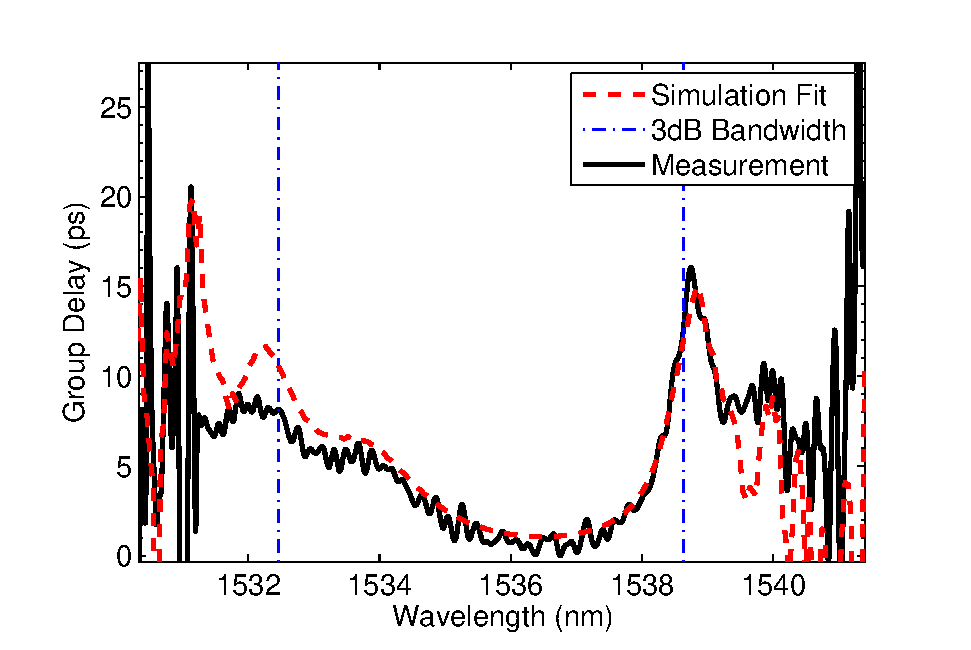
\includegraphics[width=.99\columnwidth]{data/Phase}
\caption{ Group delay response of the tunable filter at the drop port. The delay stays within 12 ps between any two points in the band. The out of band results are noisy due to the weak signal.}
\label{fig:phase}
\end{figure}


%\section{Conclusion}
In summary, we have demonstrated a bandwidth tunable filter with a low insertion loss of less then 0.5 dB, low ripples of less than 0.3 dB, a large maximal bandwidth of greater than 750 GHz, and high contrast of 55 dB. 
Compared to other devices based on microring resonators and MZIs (see Table \ref{table:comparison}), it enables a much larger maximal passband and does not suffer from small FSRs. 
A large bandwidth tuning range over 670 GHz has been achieved, which, to the best of our knowledge, is the widest ever demonstrated on a silicon chip. 
This ultra-wide bandwidth tunability makes the device very attractive for next-generation ultrahigh baud-rate applications (e.g., high-capacity super-channel transmissions) and flexible optical networking. 


\begin{table*}[t]
\caption{Recent results with multi-element on-chip silicon filters}
\begin{tabular}{cccccc}
    \hline
	Publication & Filter type & BWmax / FSR & Tunable BW & On-chip loss & Contrast \\
    \hline
    %Ibrahim (2011) &	Cascaded MRs &	0.4 GHz / 10 GHz &	0.6-2 GHz &	0.6 dB &	30 dB
    % \\
    %Alipour (2011) &	Cascaded MRs &	5 GHz / 650 Ghz &	0.8-5 GHz &	1.25-3.75 dB &	38 dB
    % \\
    Ding (2011) &	MRs + MZI &	55 GHz / 1 THz &	28-55 GHz &	3.6 dB &	30 dB
     \\
 	Orlandi (2012) &	MRs + MZI &	173 GHz / 200 GHz &	23-173 GHz &	0.46-1.06 dB &	15-34 dB
      \\
    %Luo (2012) &	Cascaded MRs &	100 GHz / 750 Ghz &	No &	0.3-0.6 dB &	50 dB  \\
    Ong (2013)\cite{ong2013ultra} &	Cascaded MRs &	125 GHz/ 0.9 THz &	11.6-125 GHz &	0.25 dB &	50-100 dB
      \\
    This work & Cascaded contra-DC &	778 GHz / Unlimited  &	117-778 GHz &	0.5 dB &	55 dB \\
    
    \hline
    \label{table:comparison}
   \end{tabular}
    \end{table*}



%\subsection{Edge roll-off / Bandwidth effectiveness}


\section*{Acknowledgments}
We acknowledge CMC Microsystems for the  software and the fabrication subsidy. We thank Yun Wang and Lukas Chrostowski with the Univeristy of British Columbia for the fiber grating coupler design. The authors acknowledge the Natural Sciences and Engineering Research Council of Canada, TeraXion and Prompt for funding this research. The silicon chip was fabricated at the University of Washington Microfabrication/Nanotechnology User Facility, a member of the NSF National Nanotechnology Infrastructure Network.

\bibliographystyle{osajnl}
\bibliography{bibli}

\end{document}